\chapter{Optimization}
\label{sec:opt}
Executing \textit{FloatingSE} by hand is sufficient to explore some simple
one-off or comparison analyses between a few runs.  OpenMDAO
provides extensive optimization capability, which can give yield richer
and more insightful analyses.

\section{Methodology}
For a full substructure optimization, we begin with the formulation of
a constrained, nonlinear single-objective optimization problem with
mixed-integer design variables,
\begin{equation}
\begin{array}{ll}
  \min & f\left(\mbf{x}\right)\\
  \text{subject to} & \mbf{g}\left(\mbf{x}\right) \leq 0,\\
  \text{and}& \mbf{x} \in \mbf{X} \\
  \end{array}
\end{equation}
where,
\begin{itemize}
\item $\mbf{x}$ is a vector of $n$ \textit{design variables}, the variables that are adjusted in order to
  find the optimal solution (see Table \ref{tbl:designvar});
\item $f(\mbf{x})$ is the nonlinear \textit{objective function}, the
  metric to be minimized by the optimization algorithm;
\item $\mbf{g} (\mbf{x})$ is the vector of \textit{inequality constraints}, the
  set of conditions that the solution must satisfy (see Table
  \ref{tbl:constraints}).  There are no equality constraints;
\item $\mbf{X}$ is the design variable \textit{bounds}, the bracket of
  allowable design variable values.
\end{itemize}

Note that this problem statement imposes no requirements on the types of
variables in $\mbf{x}$.  A mixed-integer solution is desired, where some
design variables are continuous ($x \in \mbb{R}$) and others are
discrete variables that can only take integer values ($x \in
\mbb{Z}$).  An example of an integer design variable in this
application is the number of offset columns or the number of mooring
line connections.


\section{Gradient-Based versus Derivative-Free Algorithms}
Derivative-free optimization algorithms are preferable for substructure
optimization problems for a few reasons, despite their known performance
drawbacks in terms of wall-clock time.  First, to do a complete
configuration optimization of the substructure, a mixed-integer capable
algorithm is required.  No gradient-based optimization algorithm is
capable of handling these types of variables directly (unless a rounding
approximation is used).  A genetic algorithm, properly designed, can
support mixed-integer variables for a global design space optimization.

Another reason for the selection of derivative-free algorithms is that
the \textit{FloatingSE} uses a number of third-party, black box tools or
algorithms that do not come with analytical gradients.  This includes
Frame3DD, MAP++, and some of the API 2U procedures that rely on roots of
nonlinear equations.  Thus, gradient-based optimization algorithms would
be forced to use finite difference approximations around these tools at
the very least.  However, derivatives approximated with finite
differences are expensive to compute accurately.  If computed
inaccurately, for the sake of reducing computational time, finite
difference derivatives can easily lead an optimization algorithm astray,
especially in highly nonlinear or tightly constrained regions of the
design space.  This is another reason for the use of
derivative-free algorithms, even when conducting local neighborhood
design space optimization and/or sensitivity studies.


\section{Design Variables}
In WISDEM, via OpenMDAO, any input parameter can be designated a design
variable.  The design variables used in this study focused on the
geometric specification of the floating substructure and mooring
subsystem.  Slightly different design variables and bounds were used for
spar, semisubmersible, and TLP optimizations.  The complete listing of
the design variables for each optimization configuration is shown in
Table \ref{tbl:designvar}.  Note that the integer design variables were
only used in the global optimization with the genetic algorithm, not the
local search with the simplex algorithm.


\begin{table}[htbp] \begin{center}
    \caption{Standard design variables, their size, and units used for
      optimization in \textit{FloatingSE}.  Note that $n_s$ denotes the
      number of sections in the column discretization.}
    \label{tbl:designvar}
{\footnotesize
  \begin{tabular}{ l l c l c } \hline
    \textbf{Variable} & \textbf{Name} & \textbf{Units} & \textbf{Type} & \textbf{Bounds} \\ \hline \hline
    Main col section height &\mytt{main\_section\_height}& \unit{$m$} & Float array ($n_s$) & 0.1--50 \\
    Main col outer diameter &\mytt{main\_outer\_diameter}& \unit{$m$} & Float array ($n_s+1$) &2.1--40 \\
    Main col wall thickness &\mytt{main\_wall\_thickness}& \unit{$m$} & Float array ($n_s+1$)  &0.001--0.5 \\
    Main col freeboard & \mytt{main\_freeboard}& \unit{$m$} & Float scalar &0--50 \\
    Main col stiffener web height &\mytt{main\_stiffener\_web\_height}& \unit{$m$} & Float array ($n_s$) &0.01--1 \\
    Main col stiffener web thickness &\mytt{main\_stiffener\_web\_thickness}& \unit{$m$} & Float array ($n_s$) &0.001--0.5 \\
    Main col stiffener flange width &\mytt{main\_stiffener\_flange\_width}& \unit{$m$} & Float array ($n_s$) &0.01--5 \\
    Main col stiffener flange thickness &\mytt{main\_stiffener\_flange\_thickness}& \unit{$m$} & Float array ($n_s$) &0.001--0.5 \\
    Main col stiffener spacing &\mytt{main\_stiffener\_spacing}& \unit{$m$} & Float array ($n_s$) &0.1--100 \\
    Main col permanent ballast height &\mytt{main\_permanent\_ballast\_height}& \unit{$m$} & Float scalar &0.1--50 \\
    Main col buoyancy tank diameter &\mytt{main\_buoyancy\_tank\_diameter}& \unit{$m$} & Float scalar &0--50 \\
    Main col buoyancy tank height &\mytt{main\_buoyancy\_tank\_height}& \unit{$m$} & Float scalar &0--20 \\
    Main col buoyancy tank location (fraction) &\mytt{main\_buoyancy\_tank\_location}&& Float scalar &0--1 \\
    \hline
    Number of offset cols &\mytt{number\_of\_offset\_columns}&& Integer scalar & 3-5 \\
    Offset col section height &\mytt{offset\_section\_height}& \unit{$m$} & Float array ($n_s$) &0.1--50\\
    Offset col outer diameter &\mytt{offset\_outer\_diameter}& \unit{$m$} & Float array ($n_s+1$)&1.1--40\\
    Offset col wall thickness &\mytt{offset\_wall\_thickness}& \unit{$m$} & Float array ($n_s+1$) &0.001--0.5\\
    Offset col freeboard & \mytt{offset\_freeboard}& \unit{$m$} & Float scalar &2--15 \\
    Offset col stiffener web height &\mytt{offset\_stiffener\_web\_height}& \unit{$m$} & Float array ($n_s$) &0.01--1\\
    Offset col stiffener web thickness &\mytt{offset\_stiffener\_web\_thickness}& \unit{$m$} & Float array ($n_s$) & 0.001--0.5\\
    Offset col stiffener flange width &\mytt{offset\_stiffener\_flange\_width}& \unit{$m$} & Float array ($n_s$) & 0.01--5\\
    Offset col stiffener flange thickness &\mytt{offset\_stiffener\_flange\_thickness}& \unit{$m$} & Float array ($n_s$) & 0.001--0.5\\
    Offset col stiffener spacing &\mytt{offset\_stiffener\_spacing}& \unit{$m$} & Float array ($n_s$) &0.01--100\\
    Offset col permanent ballast height &\mytt{offset\_permanent\_ballast\_height}& \unit{$m$} & Float scalar &0.1--50\\
    Offset col buoyancy tank diameter &\mytt{offset\_buoyancy\_tank\_diameter}& \unit{$m$} & Float scalar &0--50 \\
    Offset col buoyancy tank height &\mytt{offset\_buoyancy\_tank\_height}& \unit{$m$} & Float scalar &0--20 \\
    Offset col buoyancy tank location (fraction) &\mytt{main\_buoyancy\_tank\_location}&& Float scalar & 0--1 \\
    Radius to offset col &\mytt{radius\_to\_offset\_column}& \unit{$m$} & Float scalar &5--100 \\
    \hline
    Pontoon outer diameter &\mytt{pontoon\_outer\_diameter}& \unit{$m$} & Float scalar &0.1--10 \\
    Pontoon wall thickness &\mytt{pontoon\_wall\_thickness}& \unit{$m$} & Float scalar &0.01--1 \\
    Lower main-offset pontoons &\mytt{lower\_attachment\_pontoons\_int}&& Integer scalar & 0--1 \\
    Upper main-offset pontoons &\mytt{upper\_attachment\_pontoons\_int}&& Integer scalar & 0--1 \\
    Cross main-offset pontoons &\mytt{cross\_attachment\_pontoons\_int}&& Integer scalar & 0--1 \\
    Lower offset ring pontoons &\mytt{lower\_ring\_pontoons\_int}&& Integer scalar & 0--1 \\
    Upper offset ring pontoons &\mytt{upper\_ring\_pontoons\_int}&& Integer scalar & 0--1 \\
    Outer V-pontoons &\mytt{outer\_cross\_pontoons\_int}&& Integer scalar & 0--1 \\
    Main col pontoon attach lower (fraction) &\mytt{main\_pontoon\_attach\_lower}&& Float scalar & 0--0.5\\
    Main col pontoon attach upper (fraction) &\mytt{main\_pontoon\_attach\_upper}&& Float scalar & 0.5--1\\
    \hline
    Fairlead (fraction) &\mytt{fairlead\_location}&& Float scalar &0--1 \\
    Fairlead offset from col &\mytt{fairlead\_offset\_from\_shell}& \unit{$m$} & Float scalar & 5--30\\
    Fairlead pontoon diameter &\mytt{fairlead\_support\_outer\_diameter}& \unit{$m$} & Float scalar & 0.1--10 \\
    Fairlead pontoon wall thickness &\mytt{fairlead\_support\_outer\_thickness}& \unit{$m$} & Float scalar &0.001--1 \\
    Number of mooring connections &\mytt{number\_of\_mooring\_connections}&& Integer scalar &3--5 \\
    Mooring lines per connection &\mytt{mooring\_lines\_per\_connection}&& Integer scalar &1--3 \\
    Mooring diameter &\mytt{mooring\_diameter}& \unit{$m$} & Float scalar &0.05--2 \\
    Mooring line length &\mytt{mooring\_line\_length}& \unit{$m$} & Float scalar &0--3000 \\
    Anchor distance &\mytt{anchor\_radius}& \unit{$m$} & Float scalar &0--5000 \\
  \hline \end{tabular}
}
\end{center} \end{table}



\section{Constraints}
Due to the many design variables, permutations of settings, and applied
physics, there are many constraints that must be applied for an
optimization to close.  The constraints capture both physical
limitations, such as column buckling, but also inject industry
standards, guidelines, and lessons learned from engineering experience
into the optimization.  As described in Section \ref{sec:intro}, this is
a critically important element in building a MDAO framework for
conceptual design that yields feasible results worth interrogating
further with higher-fidelity tools.  The constraints used in the
substructure design optimization and sensitivity studies are listed in
Table \ref{tbl:constraints}.  Where appropriate, some of the constraint
values differ from one type of substructure to another.  Some additional
explanation is provided for a handful of constraints in the subsections
below.


\begin{table}[htbp] \begin{center}
    \caption{Optimization constraints used in \textit{FloatingSE}.}
    \label{tbl:constraints}
    {\footnotesize
  \begin{tabular}{ c l c l} \hline
    \textbf{Lower} & \textbf{Variable} & \textbf{Upper} & \textbf{Comments}\\
\hline \hline
 & \textbf{Tower / Main / Offset Columns} &  & \\
 & Eurocode global buckling & 1.0 & \\
 & Eurocode shell buckling & 1.0 & \\
 & Eurocode stress limit & 1.0 & \\
  & Manufacturability & 0.5 & Taper ratio limit\\
  120.0 & Weld-ability &  & Diameter:thickness ratio limit\\
\hline & \textbf{Main / Offset Columns} &  & \\
 & Draft ratio & 1.0 & Ratio of draft to max value\\
 & API 2U general buckling- axial loads & 1.0 & \\
 & API 2U local buckling- axial loads & 1.0 & \\
 & API 2U general buckling- external loads & 1.0 & \\
 & API 2U local buckling- external loads & 1.0 & \\
 & Wave height:freeboard ratio & 1.0 & Maximum wave height relative to freeboard\\
  1.0 & Stiffener flange compactness &  & \\
  1.0 & Stiffener web compactness &  & \\
 & Stiffener flange spacing ratio & 1.0 & Stiffener spacing relative to flange width\\
 & Stiffener radius ratio & 0.50 & Stiffener height relative to diameter\\
\hline & \textbf{Offset Columns} &  & \textit{Semi only}\\
  0.0 & Heel freeboard margin &  & Height required to stay above waterline at max heel\\
  0.0 & Heel draft margin &  & Draft required to stay submerged at max heel\\
\hline & \textbf{Pontoons} &  & \textit{Semi only}\\
 & Eurocode stress limit & 1.0 &\\
\hline & \textbf{Tower} &  & \\
  -0.01 & Hub height error & 0.01 &\\
\hline & \textbf{Mooring} &  & \\
  0.0 & Axial stress limit & 1.0 &\\
 & Line length limit & 1.0 & Loss of tension or catenary hang\\
 & Heel moment ratio & 1.0 & Ratio of overturning moment to restoring moment\\
 & Surge force ratio & 1.0 & Ratio of surge force to restoring force\\
\hline & \textbf{Geometry} &  & \\
  1.0 & Main-offset spacing &  & Minimum spacing between main and offset columns \\
  0.0 & Nacelle transition buffer &  & Tower diameter limit at nacelle junction\\
  -1.0 & Tower transition buffer & 1.0 & Diameter consistency at freeboard point\\
\hline & \textbf{Stability} &  & \\
  0.10 & Metacentric height &  & \textit{Not applied to TLPs}\\
  1.0 & Wave-Eigenmode boundary (upper) &  & Natural frequencies below wave frequency range\\
 & Wave-Eigenmode boundary (lower) & 1.0 & Natural frequencies above wave frequency range\\
  0.0 & Water ballast height limit & 1.0 & \\
  0.0 & Water ballast mass &  & Neutral buoyancy\\
    \hline \end{tabular}
  }
\end{center} \end{table}

\subsection{Geometry Constraints}
Words
%
\begin{table}[htbp] \begin{center}
    \caption{Constraint variables for the geometry in \textit{FloatingSE}.}
    \label{tbl:geomconvar}
{\footnotesize
  \begin{tabular}{l l l } \hline
    \textbf{Variable} & \textbf{Type} & \textbf{Description} \\
    \mytt{max\_draft} & Float scalar & Maximum allowable draft for the substructure\\
  \hline \end{tabular}
}
\end{center} \end{table}

\subsection{Manufacturing Constraints}
Manufacturing steel frustum shells requires rolling steel plates into
shape and welding along a seam to close the section.  To accommodate
traditional rolling and welding practices, both the diameter taper over
the course of a section and the wall thickness ratio relative to the
diameter are capped.  Similarly, to facilitate welding the
semisubmersible pontoons to the columns, constraints regarding the radio
of diameters between the two are enforced. These limits are determined
by user parameters in Table \ref{tbl:manconvar} and constraints,
%
\begin{table}[htbp] \begin{center}
    \caption{Constraint variables for the manufacturability in \textit{FloatingSE}.}
    \label{tbl:manconvar}
{\footnotesize
  \begin{tabular}{l l l } \hline
    \textbf{Variable} & \textbf{Type} & \textbf{Description} \\
    \mytt{min\_taper\_ratio} & Float scalar & For manufacturability of rolling steel\\
    \mytt{min\_diameter\_thickness\_ratio} & Float scalar & For weld-ability\\
    \mytt{connection\_ratio\_max} & Float scalar & For welding pontoons to columns\\
  \hline \end{tabular}
}
\end{center} \end{table}

\subsection{Stress Limits and Code Compliance}
The stress and buckling code compliance constraints are formulated as
utilization ratios (ratio of actual to maximum values), with a safety
factor, which must be less than one. The safety factor parameters are
listed in Table \ref{tbl:safetyvar}.
%
\begin{table}[htbp] \begin{center}
    \caption{Variables specifying the factors of safety within \textit{FloatingSE}.}
    \label{tbl:safetyvar}
{\footnotesize
  \begin{tabular}{ l l l } \hline
    \textbf{Variable} & \textbf{Type} & \textbf{Description} \\
    \mytt{gamma\_f} & Float scalar & Safety factor on \\
    \mytt{gamma\_b} & Float scalar & Safety factor on buckling\\
    \mytt{gamma\_m} & Float scalar & Safety factor on materials\\
    \mytt{gamma\_n} & Float scalar & Safety factor on consequence of failure\\
    \mytt{gamma\_fatigue} & Float scalar & Not currently used\\
  \hline \end{tabular}
}
\end{center} \end{table}

\subsection{Stability}
As described above, surge and pitch stability are enforced through
similar approaches.  The total force and moment acting on the turbine
are compared to the restoring forces and moments applied by the mooring
system, buoyancy, or other sources at the maximum allowable point of
displacement.  These constraints are formulated as ratios with the user
specifying the maximum allowable limits via the variables in Table
\ref{tbl:moorcon}.
%
\begin{table}[htbp] \begin{center}
    \caption{Constraint variables for the mooring system in \textit{FloatingSE}.}
    \label{tbl:moorcon}
{\footnotesize
  \begin{tabular}{ l l c l } \hline
    \textbf{Variable} & \textbf{Type} & \textbf{Units} & \textbf{Description} \\
    \mytt{max\_offset} & Float scalar & $m$& Max surge/sway offset \\
    \mytt{operational\_heel} & Float scalar & $deg$& Max heel (pitching) angle in operating conditions \\
    \mytt{max\_survival\_heel} & Float scalar & $deg$& Max heel (pitching) angle in parked conditions \\
  \hline \end{tabular}
}
\end{center} \end{table}

\section{Objectives}
Different anaylses will emphasize different metrics, requiring different
objective functions.  Under the default assumption that the user wishes
to minimize cost and adhere to stability constraints, the objective
function would be total substructure cost (variable name,
\texttt{total\_cost}) or mass (variable name, \texttt{total\_mass}).

\section{Example}

\begin{figure}[htb]
  \begin{subfigure}[b]{0.29\linewidth}
    \centering 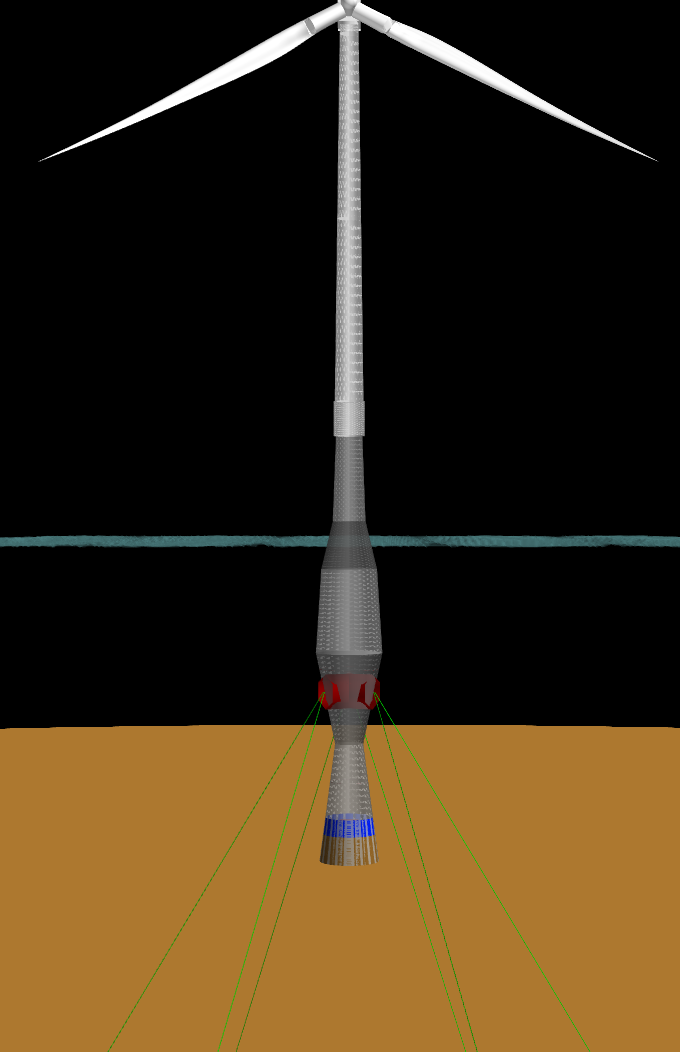
\includegraphics[width=\linewidth]{figs/spar-cost1.png}
    \caption{Spar}
  \end{subfigure}
  \begin{subfigure}[b]{0.39\linewidth}
    \centering 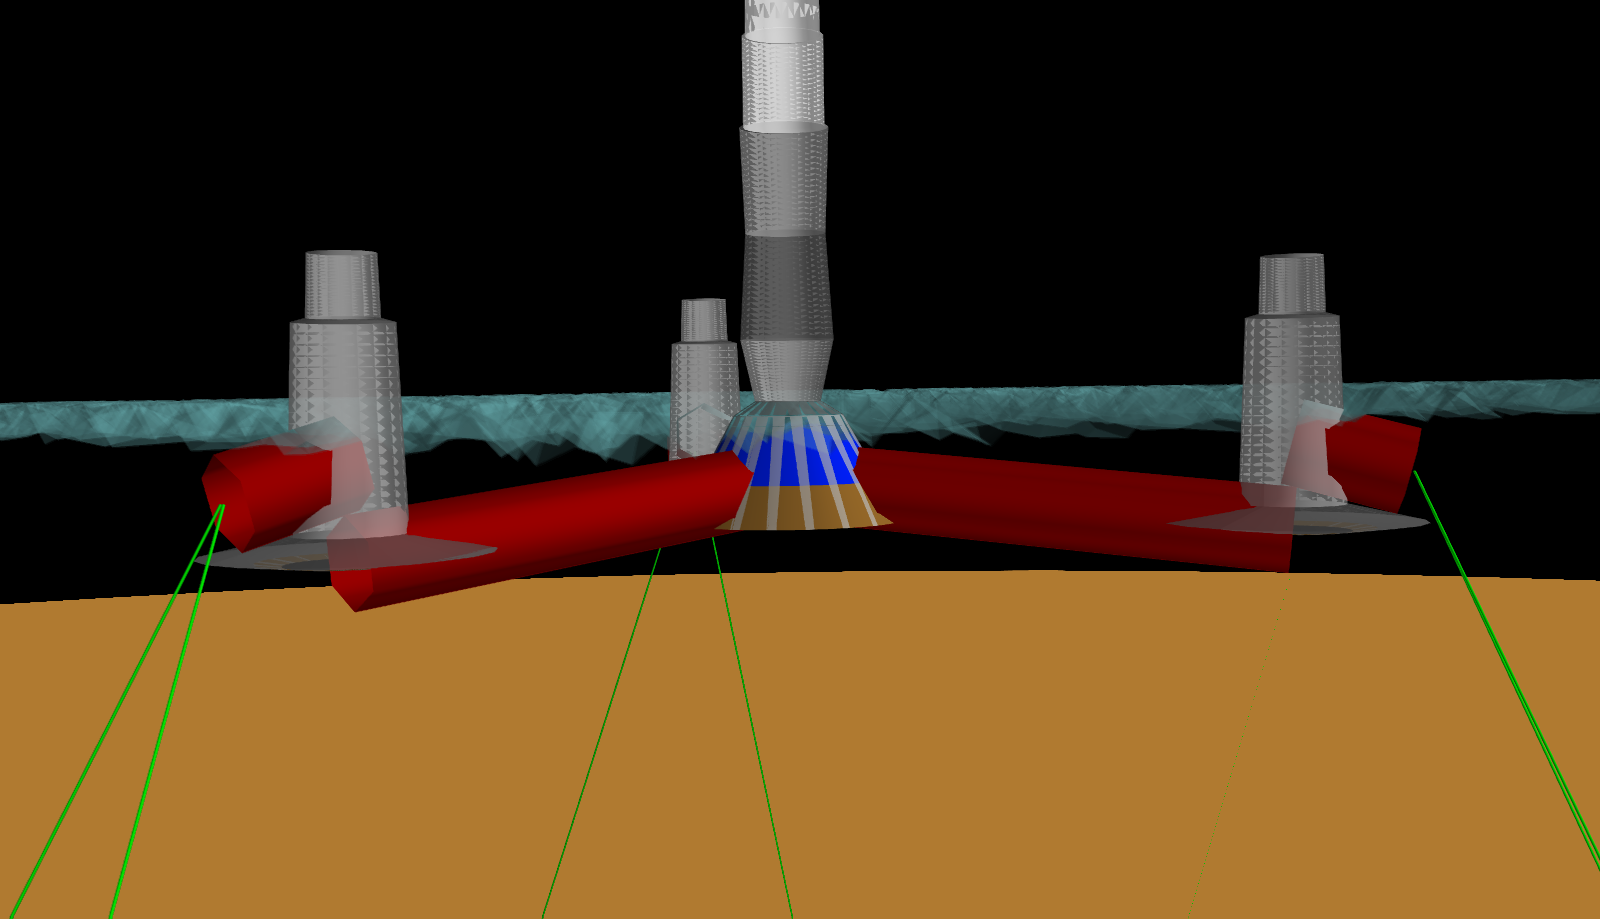
\includegraphics[width=\linewidth]{figs/semi-mass2.png}
    \caption{Semisubmersible}
  \end{subfigure}\\
  \begin{subfigure}[b]{0.29\linewidth}
    \centering 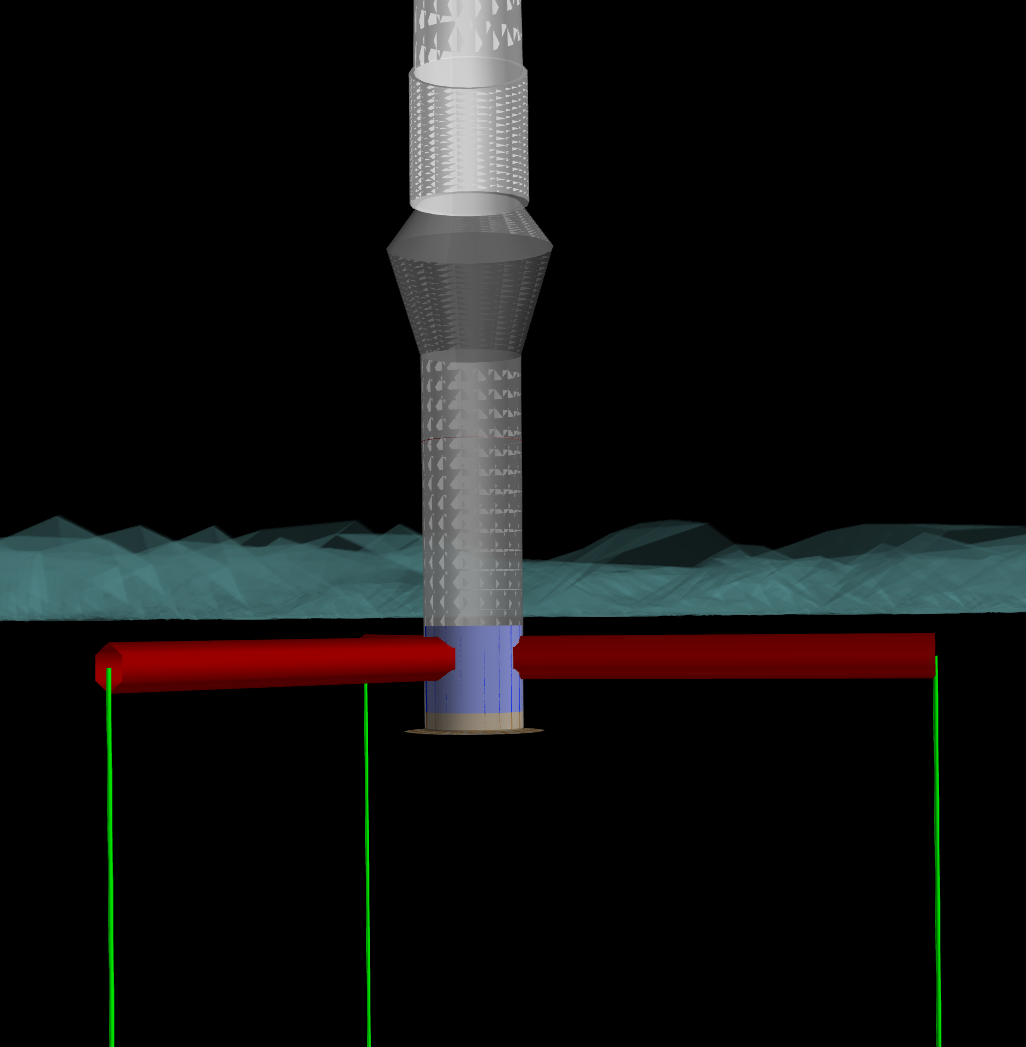
\includegraphics[width=\linewidth]{figs/tlp-cost2.png}
    \caption{Spar}
  \end{subfigure}
  \caption{Examples of optimized spar, semisubmersible, and TLP geometries.}
  \label{fig:optex}
\end{figure}

